% METHODOLOGY CHAPTER
\chapter{Methodology}\label{ch:methodology}

In this chapter, the methodology that is used to research the topic is presented.
This study attempts to produce a predictive analytics model that uses a machine learning approach that can predict the match outcomes of a League of Legends match.
Firstly, an explanation of the pre-processing data-pipeline - how the data was collected, a description of the dataset, and how the data is prepared and cleansed for modelling.
The subsequent section then follows the dataset through the prediction methodology, and ends with how the predictive capability of the model is tested and assessed.

\section{Philosophy, Approach and Strategy}\label{sec:Research Philosophy}

This section outlines the research philosophy under which the research is conducted, and how the methodology will be approached during the course of this study.
The framework behind the methodology explored during this section is built upon the works of~\citet{saunders2007research}.
They proposed a methodological framework made up of 6 steps, that underpin any piece of research that they labelled the `research onion'.
This dissertation will mostly follow the research philosophy of pragmatism, this ideology aims to find more of a practical point of view where both subjectivity and objectivity matter, and form a practical combination of methods that will be used to ultimately answer the research questions.
The approach to the research will be quantitative, and mainly follow a deductive approach, with the work completed being based upon previous theories and conclusions that previous researchers have created.
This approach will mean that there will be analysis of numerical results, that are specific to the situation using statistical modelling and mathematics.
The strategy applied to this research will be a mono-method experimental research strategy.
This involves manipulating independent variables to observe a change in the dependent variable, in order to determine the relationship between the variables in a dataset.

\section{Data Pre-processing}\label{sec:Data Pre-processing}
\subsection{Data Overview}\label{subsec:Data Overview}
The data used in this project is based upon the match data collected from all the League of Legends esports leagues found globally in 2021.
Oracle's Elixir is a website that collects all the esports match data provided by Riot Games;
the publisher of League of Legends, and aggregates them into datasets that are freely downloadable and offered to coaches, analysts and fans alike~\citep{oraclesElixir}.
These datasets are updated daily, and go back until 2014.
When the dataset is downloaded, it is given in a .csv format that can be opened Microsoft Excel to get an easier perspective of the data.
Once opened, it can be seen that it is a huge dataset contained within one spreadsheet with 149,496 rows and 123 columns, and will have to be prepared in order to be ready for  modelling.
The rows contain data from a unique player within a given match, this starts off with the Blue side Top Lane player and continues serially until the Red side Support player is reached, it will then contain a row for each team's collective data.
This means there are 12 rows for each unique match before reaching data for the next match, this can be seen in Table~\ref{tab:1}.

\begin{table}[h!]
\centering
\caption{An excerpt from the dataset.}
\begin{tabular}{ c c c c }
 \hline
 Participant & Side & Position & TeamName \\ [0.5ex]
 \hline
 1 & Blue & top & DWG KIA \\
 2 & Blue & jng & DWG KIA \\
 3 & Blue & mid & DWG KIA \\
 4 & Blue & bot & DWG KIA \\
 5 & Blue & sup & DWG KIA \\
 6 & Red & top & Nongshim RedForce \\
 7 & Red & jng & Nongshim RedForce \\
 8 & Red & mid & Nongshim RedForce \\
 9 & Red & bot & Nongshim RedForce \\
 10 & Red & sup & Nongshim RedForce \\
 100 & Blue & team & DWG KIA \\
 200 & Red & team & Nongshim RedForce \\ [1ex]
 \hline
\end{tabular}
\label{tab:1}
\end{table}

The target variable is the intended prediction variable, and is found at the eighteenth column named `Result'.
It is a binary value and simply denotes whether a team wins or loses using 1 and 0 respectively.
Preceding this column are the match descriptor variables, here lies the unique match id, the league in which the game is played, the date, the game number for best of 5 series, and other information such as match length and those found in Table~\ref{tab:1}.
One of the key columns that will be used is the `datacompleteness' variable, this contains 4 options of `complete', `found', `partial' and `reparse', and describes the state of the data in a given row.
Following these 18 match descriptor variables, are the 105 in-game statistic variables that have been recorded.
The values in these columns will be the key predictors in our match-outcome prediction model, however the usefulness of each variable will be decided later in Section~\ref{subsec:Data Preparation}.
These predictors range from simple statistics such as the total number of kills or deaths in a given match, to more advanced statistics such as GSPD - The average gold spent difference between teams.
Many of these statistics also come in the form such as `goldat10' and `goldat15', which is simply the amount of gold obtained by the 10 and 15-minute mark in-game respectively.
These time-based statistics will be important in factoring how much the match outcome varies by the in-game time.
Another note about the data, is the fact that it tracks the opponent statistics for all of these statistics inside each row, so this should allow the use of data from only one side whilst maintaining all the statistics from both teams.

\subsection{Data Preparation}\label{subsec:Data Preparation}
It is vital for the data gathered to be both reliable and of high validity, this is ensured by a rigorous data preparation stage.
In order for the data to be prepared for modelling, coding is required.
The coding language used in this study is Python, it is a well-rounded language that is opensource and allows access to great analytical libraries, visualisations and is well documented online whilst being the main analytics language used in industry~\citep{tiobePython}.
Jupyter Notebooks are used as a personal preference, but any IDE could be used. \\

The CSV file of all the match data for 2021 is read into the notebook as a dataframe.
The data-types of the dataframe are checked to ensure that they are as intended.
Once again the data is inspected and a large proportion of missing data becomes visible, many features such as `turretplates' and `elementaldrakes' had well over 100,000 null values and were not fully complete.
Features like these will likely be removed during feature selection due to their lack of data, otherwise it would ultimately harm the modelling process - the feature selection process will be covered later.
Firstly, the dataframe is sorted for the feature `datacompleteness' and opts to reject any row that is not `complete', this massively helps reduce the number of null values found in the data.
Additionally, another filter is used on the `position' feature, reducing our data to only rows with team information instead of a mixture of individual and team data.
This will help focus on the overall impact of the team's actions in response to an outcome of a match.
Now the dataframe should only consist of team-base data, but will contain rows for both the blue-side and the red-side teams for each individual `gameid'.
The problem here is that only one side of data is required to predict with, here it is chosen to predict the outcome of a blue-side team using blue-side match data.
This issue is easily subverted by dropping any duplicate `gameid' rows, leaving the dataframe with only team-based data from the blue-side team.
As the dataset is now made-up of only team-based data, no duplicate rows exist and contains no null values, descriptive statistics are used to further inspect the data to search for potential outliers that could corrupt our model.
This is completed using the `describe' function and manually searching for data minimums and maximums that look suspicious.
It can be seen that the `gamelength' feature has an unusually high maximum value when compared to both the median value and the 75th percentile value.
This is then removed by removing any rows that exist above the 99th percentile for `gamelength', reducing the maximum gamelength from over 40,700 minutes, down to a maximum of 47.2 minutes;
a gamelength that is as expected.
After these steps are complete, the dataset has been properly cleansed and now 11,145 rows remain.\\

Then comes the step of feature selection that aims to reduce the overall dimensionality of the dataset, increase the computational cost of modelling and to improve the performance of the model~\citep{brownlee2019choose}.
All the features that include opposition team data are removed as they will cause issues with multicollinearity later, as well as prediction from opposition statistics being deemed redundant for understanding how a given team could improve.
After removing many redundant features, a correlation matrix is created between the remaining features in the data subset.
Finding the correlation allows for the measure of how features share an interdependence between one another.
Here the Kendall correlation is calculated between features using the `corr()' function and visualised using the `heatmap()' function from the `Seaborn' package.
Correlation values between the target and themselves are deemed better predictors when this value moves closer to 1 or -1.
Therefore, those features with values close to zero should be removed from the dataset as they likely provide no benefit to the model, whilst adding further complexity.
On the contrary, features with high correlation values with other predicting features should be removed or reworked due to the issue of multicollinearity~\citep{alin2010multicollinearity}.
If not dealt with, this causes problems when trying to interpret what features actually are influential on the output of a model.  \\

The correlation matrix can be found at Appendix~\ref{fig:CorrMat1}.
Here it can be observed that the correlations with our target - `result', range anywhere between an absolute minimum value of 0.17 from the `firstdragon' and `assistsat10' features, to 0.66 from the `firstbaron' variable.
These correlations suggest that most features have a weak-moderate, with a few stronger predictors such as `firstbaron' and `firstthreetowers'.
When the correlation between features is examined, features containing assists and kills at the 10 and 15 minute mark are highly positively correlated with a values of 0.80 and 0.78.
When correlations are high between features, these features should be either be ignored or transformed.
Here another test for multicollinearity is also used, called the Variance Inflation Factors or VIF\@.
This tests each feature for how much variance the feature adds to the overall variance of the model, and generally describes how collinear a feature is with its other features.
The results can be seen in Table~\ref{tab:VIF}, where it is deemed that any variable above 10 may be an issue.

\begin{table}[h]
    \centering
    \caption{A table showing the results of the VIF test}
    \begin{tabular}{l c c}
        \toprule
        \textbf{Feature Name} & \textbf{VIF Before} & \textbf{VIF After} \\
        \midrule
            playoffs &	1.217690  & 1.235018 \\
            patch &	12.464378  & 3.160019 \\
            gamelength &	1.006723 & 8.216505 \\
            firstblood &	2.814385  & 2.447549 \\
            firstdragon &	1.876673  & 1.804742 \\
            firstherald &	4.543882  & 3.472183 \\
            firstbaron &	2.484599 & 2.493748 \\
            firsttower &	4.868430 & 3.944228 \\
            firstmidtower &	4.583104 & 4.571757 \\
            firsttothreetowers &	5.468883 & 5.380049 \\
            golddiffat10 &	15.818089 & - \\
            xpdiffat10 &	8.758268 & - \\
            csdiffat10 &	13.385455 & 4.371368  \\
            killsat10 &	54.651732 & - \\
            assistsat10 &	18.985235 & - \\
            deathsat10 &	30.215561 & 8.042111  \\
            golddiffat15 &	20.547368 & - \\
            xpdiffat15 &	17.244354 & - \\
            csdiffat15 &	16.369323 & 4.886503  \\
            killsat15 &	76.322270 & - \\
            assistsat15 &	27.789294 & - \\
            deathsat15 &	40.345937 & 9.899573  \\
            KillParat10 & - & 6.116191 \\
            KillParat15 & - & 7.917371 \\
        \bottomrule
    \end{tabular}
    \label{tab:VIF}
\end{table}



Here a feature is deemed an issue if its VIF value exceeds 10, which many variables do - including those that also have large correlation values.
Using the knowledge gained from both these tests, it is chosen to transform the kill and assist features, as they both are deemed useful to the model due to their correlation to the target variable.
The `xpdiff' and `golddiff' features will also be removed.
These four features will simply be combined to create two new features called `KillParat10' and `KillParat15', and were constructed as such:

\[ Kill \: Participations = Kills + Assists \]

Checking the correlation of these new features now shows that the relationship between the target remains stable, whilst removing the problematic large correlations between predictor features in the dataset.
The VIF test is then repeated to ensure that the dataset no longer contains any potential multicollinearity issues, and every feature passes with a sub-10 VIF as seen in Table~\ref{tab:VIF}.
Another correlation issue is seen between recurrent features at different minute intervals in-game.
This is fixed by splitting these features into different datasets which in-turn will create separate models based on the statistics from the 10-minute mark, the 15-minute mark and the 20-minute mark.
A description of the data found across all three data subsets can be seen in Table~\ref{tab:DataDescription}. \\

\begin{table}[h]
    \centering
    \caption{A table describing the data found within the dataset}
    \begin{tabular}{p{0.35\linewidth} p{0.6\linewidth}}
        \toprule
        \textbf{Feature Name} & \textbf{Description} \\
        \midrule
        Playoffs & If the match is a playoff game  \\
        Patch & The game patch the match is played on  \\
        Gamelength & The duration the game was played  \\
        First Blood & If the first kill was obtained by the blue team   \\
        First Dragon & If the first Dragon of the match was slain by the blue team   \\
        First Herald & If the first Herald of the match was slain by the blue team    \\
        First Baron & If the first Baron of the match was slain by the blue team   \\
        First Tower & If the first Tower of the match was destroyed by the blue team    \\
        First Mid Tower & If the first Mid-lane Tower of the match was slain by the blue team \\
        First to Three Towers & If the first three Towers of the match were destroyed by the blue team  \\
        CS Diff at X & The differential in number of minions slain between the teams at a given interval  \\
        Deaths at X & The number of deaths by the blue team at a given interval \\
        Kill Participations at X & The number of kill participations of the blue team at a given interval  \\
        \bottomrule
    \end{tabular}
    \label{tab:DataDescription}
\end{table}


Balancing the data was deemed unnecessary due to the target variable - `result', having a 52.8 - 47.2\% win to loss balance as seen in Figure~\ref{fig:DataBalance}.
This means that the dataset does not require any balancing techniques such as SMOTE to be applied, as it already should give reliable and decisive outputs.

\begin{figure}[h!]
    \centering
    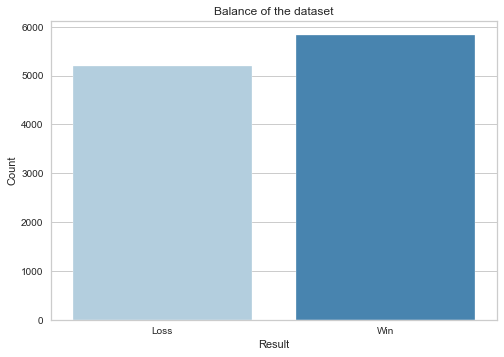
\includegraphics[width=0.9\textwidth]{figures/DataBalance}
    \caption{A graph showing the target balance of the dataset}
    \label{fig:DataBalance}
\end{figure}

Finally, the data is put through the normalization process, re-scaling the data in each column between the values of 0 and 1.
This step is completed to reduce the effects of the magnitude of feature scale on the model, potentially creating faster converging and better performing models~\citep{normalizePython}.

\section{Data Modelling}\label{sec:Data Modelling}
Now that the dataset has been properly collected, cleansed and processed, the data can enter the data modelling process.
With this data the target is a binary classification problem, meaning that a classification algorithm is required to help generate a probability for our target variable based on our features.
As mentioned in Section~\ref{ch:literaturereview}, previous works have used a variety of methods such as Naïve Bayes classifiers, the Random Forest algorithm, Recurrent Neural Networks and Gradient Boosting.
For this instance, it is chosen to use the Python Libraries - `scikit-learn' and `pycaret', they both offer a wide range of machine learning techniques
After reviewing the possible models, it was chosen that the Random Forest algorithm would be used to create the baseline model.
Then the PyCaret library would be used to test a larger pool of techniques and ultimately tune the model until the final model is chosen.
The Random Forest algorithm is a commonly used supervised machine learning algorithm that creates an ensemble of decision trees and uses a bagging, majority voting system to help classify our problem - see Figure~\ref{fig:RandomForest}.
This technique ensures that the chance of overfitting is kept to a minimum, as well as allowing for easy determination of importance from any given feature in the model.

\begin{figure}[h!]
    \centering
    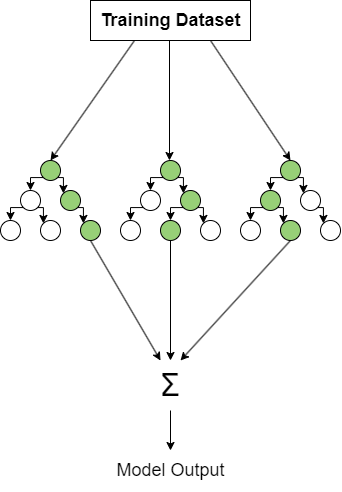
\includegraphics[width=0.5\textwidth]{figures/RandomForest}
    \caption{A diagram showing how the Random Forest algorithm classifies}
    \label{fig:RandomForest}
\end{figure}

A binary logistic regression model was also developed following the Random Forest Model.
Like the previous model, a logistic regression classifier can estimate the probability of a target binary response variable using a set of predictor variables.
This machine learning technique is based upon the natural logarithm of the odds;
commonly referred to as a logit or log-odds, system for each event with a logistic function converting these log-odds into a probability.
This logistic function is a sigmoid function that takes inputs between the bound of zero and one, it is defined as follows:

\[ p(x) = \frac{1}{1 + e^{-(\beta_0 + \beta_1 x)}} \]

Here \(\beta_{0}\) is the intercept from the linear regression equation which is solved using numerical methods, and \(\beta_{1}x\) is the regression coefficient.
With \(x\) being a combination of values from the predictor variables.
Once solved for \(p(x)\), it will provide the probability for the Blue-side team winning a given match. \\

The data then needs to be split into training data and testing data.
Here a subset of the total dataset is split purely to train the machine learning model, before it is deployed to unseen training data.
This help guarantees the model ensuring that there is no overfitting to the seen data, and validates the quality of the model.
The data split ratio is chosen at a 70:30 train-test data split.
This allows a larger split to train the model, and the test data will be tested on a more robust, accurate model because of this.
A technique called Stratified K-Fold cross validation is used to get an accurate representation of the overall population balance from the target variable - reflecting the 52.8 - 47.2\% win-loss balance, as well as evaluating a truer accuracy by summarising models built upon K subsets of data.
This leads to a model that is less biased overall and more realistic in its prediction accuracies. \\

\begin{table}[h!]
\centering
\caption{A table describing the models that were built}
\begin{tabular}{ c c c }
 \hline
 Model & Technique & Dataset \\ [0.5ex]
 \hline
 1 & Logistic Regression & 10-minute \\
 2 & Logistic Regression & 15-minute \\
 3 & Gradient Boosting Classifier & 20-minute \\[1ex]
 \hline
\end{tabular}
\label{tab:ModelsBuilt}
\end{table}

Table~\ref{tab:ModelsBuilt} shows the three models which were built for analysis purposes.
The first two models were built using the Logistic Regression with the 10, and the 15 minute datasets, and the final model was built with the Gradient Boosting Classifier using the 20 minute dataset. \\

\section{Summary}\label{sec:MethodSummary}
In this Chapter, the data extracted from Oracle's Elixir was explored and described in a data overview.
The methodology behind the data preparation were rationalised during the data cleansing and pre-processing subsections, highlighting key techniques used to ensure the data modelling process would work correctly.
This helped reduce the dataset from over 140,000 rows with 100+ features to a more succinct and useful 11,000 rows with less than 20 features.
This was then followed by the data modelling subsection, that explained the machine learning techniques used to create the predictive modelling system.
Following this chapter is Chapter~\ref{ch:resultsandanalysis}, which will present and analyse the results of this work.

